\documentclass[12pt,a4paper]{article}

% ---------- Кодировка и язык ----------
\usepackage[T2A]{fontenc}
\usepackage[utf8]{inputenc}
\usepackage[english,russian]{babel}

% ---------- Вёрстка ----------
\usepackage[margin=2.5cm]{geometry}
\usepackage{indentfirst}
\usepackage{setspace}
\usepackage{titlesec}
\newcommand{\sectionbreak}{\clearpage}
\onehalfspacing

\usepackage{paracol}
\setlength{\columnsep}{1cm} 

\usepackage{epigraph}


% ---------- Математика, графика, таблицы ----------
\usepackage{amsmath,amssymb}
\usepackage{graphicx}
\usepackage{booktabs}

% ---------- Листинги кода ----------
\usepackage{listings}
\lstset{
  basicstyle=\ttfamily\small,
  breaklines=true,
  frame=single,
  numbers=left,
  numberstyle=\tiny,
  captionpos=b,
  showstringspaces=false
}

% ---------- Ссылки ----------
\usepackage[hidelinks]{hyperref}

% ---------- Библиография ----------
% Для оформления по ГОСТ можно заменить style=numeric на style=gost-numeric
% (требуется пакет biblatex-gost).
\usepackage[
  backend=biber,
  style=gost-numeric,
  language=auto,     % язык берётся из поля langid каждой записи
  autolang=other,    % корректная работа со смешанной (рус/англ) библиографией
  sorting=none       % порядок источников: по первому упоминанию в тексте
]{biblatex}
\addbibresource{refs.bib}

% ---------- Титул ----------
\title{Отбор "LSM-дерево с нуля"}
\author{Алексеев Дмитрий Викторович \\ \small БПМИ-253 / ФКН ВШЭ \\ \small \texttt{dmivikalekseev@edu.hse.ru}}
\date{\today}

\begin{document}

\maketitle

\tableofcontents
\section{О себе}
\subsection{Навыки/Опыт/известные алгоритмы}
Так как довольно просто выполнить тестовое на хорошем уровне из-за существования LLM, я вынужден написать подробный блок о себе

В данный момент я обучаюсь на потоке М+П+ ФКН ПМИ.

В силу отличной учебы на пилотном курсе АиСД-1 (Итоговая оценка: 9), оценка по АиСД-2 пока неизвестна, но я планирую так же получить отл. 9. я знаком с большинством стандартных продвинутых алгоритмов (в частности нужные для LSM дерева фильтр Блюма и Skip-List). Отдельно перечислю известные алгоритмы во внешней памяти: List ranking за $O(Sort(n))$, B/$B^+$-дерево, Куча во внешней памяти за $O(\frac1B \lceil \log_{M/B} \frac{q}{M} \rceil)$ на запрос, BFS во внешней памяти за $O(Sort(E) + V)$, поиск компонент связности за $O(Sort(E+V)\log V)$

Так же, я люблю много писать на С++ и достаточно хорошо им владею (закончил пилотный курс на 10, и продолжаю учится на продвинутом курсе сейчас). Есть опыт разработки больших проектов: написал свой интерепретатор для некоторого ЯП \cite{interpretator}. Так же, приведу ниже менее масштабные pet-проекты:

\begin{enumerate}
    \item Интерактивные деревья поиска \cite{bstgarden}
    \item Программа для обработки фото \cite{imageprocessor} (вообще говоря, это был общекурсовой проект, но я тут заморочился с ООП, так что считаю необходимым это здесь прикрепить), p.s. все файлы сгружены в кучу, потому что тест система иначе не принимала
\end{enumerate}


\subsection{Чем вызван интерес}

Мне очень понравились задачи во внешней памяти, которые нам предложили на курсе алгоритмов. И вообще меня заинтересовала разработка каких-то структур во внешней памяти, а данная тема для курсовой позволит мне реализовать данное желание


\section {Существующие LSM-деревья}

Данный раздел посвящён тому, какие вариации внутреннего устройства имеет LSM-дерево, для чего нужны те или иные модификации, а так же в каких реальных системах управления базами данных они используются. 

Сначала давайте обсудим некоторые допущения, которые будем использовать в рассуждениях ниже.
Источник \cite{luo2020lsm} утверждает, что для LSM-дерева под стабильной нагрузкой (когда количество слоёв не меняется), перфоманс записи оптимален, когда для любого $L$ максимальный количество ключей на $L + 1$ уровне в $T$ раз больше, чем максимальное количество ключей на $L$ уровне. 

% \subsection{Дисковые компоненты}

% В LSM-деревьях может быть по разному устроено хранение дисковых компонент
% \begin{paracol}{2}
%   %TODO сделать не так категорично
%   \begin{center}\bfseries $B^+$ -дерево\end{center}
%   Используя данный метод мы во многом теряем два главных плюса LSM - дерева -- мало чтений со случайного места в диске и отказоустойчивость, потому что LSM - дерево с SSTable внедрялось, как альтернатива $B^+$-дерева, с такими свойствами. Так же амортизированно получается более долгая вставка и удаление. Единственный очевидный плюс: мы можем не хранить разные версии одного ключа, проверяя его наличие в компонентах LSM-дерева, и явно перезаписывать/удалять. данная идея изначально кажется странной, но авторы вот этой статьи \cite{luo2020lsm} вскользь упоминают данную реализацию, поэтому она стоит упоминания.
% \switchcolumn
%   \begin{center}\bfseries SSTable\end{center}
%   В такой реализации мы получаем от 
%   LSM дерева все те качества, которые и хотели получить: мало случайных I/O запросов при записи новых элементов, и слиянии существующих компонентов 
%   LSM - дерева. Отказоустойчивость: корректность записи одного элемента на диск довольно просто отследить и исправить, по сравнению с перестройкой $B^+$-дерева. С другой стороны, любые слияние таблиц происходят в дополнительной памяти, поэтому данные в таблицах никогда не будут испорчены.
% \end{paracol}
%   Так же в этой статье упоминаются различия в 

\subsection{Политика слияния}

LSM-деревья различаются между собой по политике слияния дисковых компонент. \cite{luo2020lsm} На практике обычно используют следующие две политики, каждая заточена под свой преобладающий тип запросов:

\begin{paracol}{2}
  \begin{center}\bfseries Leveling Merge Policy\end{center}

  Данная политика хранит компоненты следующим образом:

  На каждом уровне будет хранится ровно одна компонента.

  Максимальный объем компоненты на уровне $L$ хранит в $T$ раз больше ключей, чем компонента на уровне $L - 1$. Тогда компонента на слое $L$ сольется с компонентой на $L - 1$  слое много раз (в точности $T$) перед тем, как переполнится и начнёт сливаться с компонентой на слое $L + 1$.

  Как итог, Leveling Merge Policy хранит "мало" компонент (по сравнению со второй политикой), благодаря чему, показывает лучший перфоманс на запросах чтения. 

  
\switchcolumn
  \begin{center}\bfseries Tiering Merge Policy\end{center}

  Пусть вместимость $L-1$ слоя $P$ - ключей, тогда
  эта политика, на каждом слое $L - 1$ будет хранится не более $T$ компонент, каждая размера $\frac{P}{T}$ с возможно пересекающимся диапазоном ключей. Когда на слое наберётся $T$ заполненных компонент, сольем их в одну компоненту и положим на следующий уровень. Действительно, такое поведение будет корректным, потому что компонента на $L$ слое вместит в себя $T$ раз больше ключей, т.е. $P$, и максимальная вместительность уровня $L$ в точности $P \cdot T$, что в $T$ раз больше, чем на предыдущем уровне. И заполненный $L-1$ уровень станет ровно одной компонентой на $L$ слое.

  Эта политика, напротив, оптимизирована для запросов записи, за счёт снижения числа тяжёлых слияний, когда структуре приходится сливать старшие уровни.


\end{paracol}




Вообще говоря, классической политикой для LSM-дерева является именно Leveling Merge Policy, но параллельно LSM-дереву,  Jagadish и др. в своей статье \cite{jagadish1997incremental} представили очень похожую на LSMT структуру, оптимизированую под запросы записи, в которой применили "stepped-merge policy". Которая в последствии превратилась в Tiering Merge Policy, используемую в современных СУБД.


\subsection{Some Well-Known Optimizations}

\epigraph{Название данной секции дословно ссылается на название секции из статьи: "LSM-based Storage Techniques: A Survey" \cite{luo2020lsm} }

\subsubsection{Фильтр Блюма и подобные}

Фильтр Блюма - вероятностный алгоритм, для проверки принадлежности элемента множеству, гарантирующий отсутствие ложно-отрицательных срабатываний.

Устройство фильтра: есть фиксированное $m$ - количество битов и $k$ и $k$ хэш функций $h_1, \ldots, h_k $, из некоторого семейства, $h_i:\mathcal{K}\rightarrow \{0, \ldots, m-1 \}$. Положим массив $A$ битов размера $m$. Когда в множество добавляется новый ключ $K$, положим $\forall i \in \{1, \ldots, k\} A[h_i(K)] := 1$. Проверка принадлежности ключа множеству проводится следующим образом: необходимо проверить, что $\forall i A[h_i(K)] == 1$.


Фильтр Блюма позволяет проверить отсутствие ключа в SSTable, перед началом дорого (с точки зрения числа I/O запросов) поиска ключа в самой таблице. В свою очередь, ложно-положительные срабатывания не влияют на корректность ответа, только лишь добавляют расходы на поиск внутри самой компоненты. Вероятность такого  ложно-положительного срабатывания фильтра не превосходит $(1 - e ^ {-kn / m})^k$, тогда оптимальное количество хэш  функций для минимизации ошибки достигается при $k:=\frac{m}{2}\ln 2$, что на практике оказывается ~10 и позволяет достичь $1\%$ ложно-положительных срабатываний. А так как фильтр Блюма очень маленький и может быть загружен в оперативную память, накладные расходы на $I/O$ запросы к диску во многих сценариях получается существенно сократить.

Собственно, идея о том, что с помощью некоторой небольшой вероятностной структуры можно с хорошей точностью быстро проверить отсутствие ключа (если ключа нет в таблице, то структура должна гарантированно это сообщить) в одной компоненте, находит применение во многих современных СУБД. LevelDB использует встроенный фильтр Блюма - NewBloomFilterPolicy \cite{leveldbgit}. А RocksDB позволяет выбирать фильтр: NewBloomFilterPolicy, NewRibbonFilterPolicy (Ribbon Filter - некоторый аналог фильтра блюма, который занимает меньше памяти).
 \cite{rocksdbgit}.


\subsubsection{Partitioning}

%TODO я не хочу это писать


\subsection{LevelDB}

\subsection{RocksDB}

\subsection{Apache Cassandra / ScyllaDB}

\subsection{Apache HBase}

\subsection{CockroachDB}

\subsection{WiredTiger}



\section{Существующие Бенчмарки}

\subsection{YCSB}

\subsection{db\_bench}



\section{Бенчмаркинг}


\subsection{Тесты RocksDB}

\subsubsection{Пермонас записи}

В данном подразделе проведём эксперименты по перфомансу записи в зависимости от способа организации SSTable и количества ядер предоставленных RocksDB. Сравнение проводится на виртуальной машине \ref{vm:first} во встроенном в RocksDB бенчмарке db\_bench \cite{dbbench}. При следующих настройках: 


\begin{lstlisting}[language=bash, numbers=none, upquote=true]
$ db_bench \
          >out
          --benchmarks=fillrandom \
          --db=/tmp/rocks-level\
          --key_size=16\
          --value_size=984\
          --num=+ 10^7 / threads_cnt \
          --compaction_style=merge_policy \
          --threads=threads_cnt;

\end{lstlisting}


Тут представлен больше псевдокод общий для всех запусков. Все конфигурации количества потоков и политики слияния (compaction\_style) запускаются на одном и том же число запросов случайной записи (с точностью на +-8).

В этом эксперименте мы будем тестировать перфоманс случайной записи в зависимости от количества ядер при разных политиках слияния.

compaction\_style, =0 - реализует рассмотренную выше Leveling Merge Policy, а =1 - некоторая universal compaction, которая согласно документации RocksDB\cite{rocksdbwiki} "иногда называется tiered" \ , т.е. эта политика некотрый аналог выше рассмотренной Tiering Merge Policy.


\begin{figure}[ht]
  \centering
  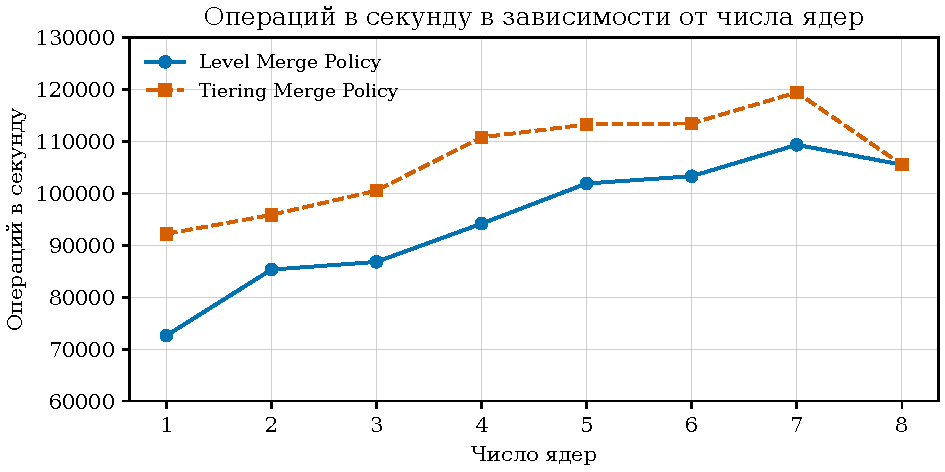
\includegraphics[width=\linewidth]{figures/04-01-ops-p-s-10-7.pdf}
  \caption{Число записей в секунду при $10^7$ операций случайной записи}\label{fig:intro-имя}
\end{figure}

Из графиков видно сразу несколько фактов:

Во-первых, не стоит отдавать СУБД все ядра системы, так как OS так же потребляет ресурсы компьютера, поэтому использование всех ядер ВМ \ref{vm:first} ведёт к снижению перфоманса.

Во-вторых, использование большего числа потоков записи всё ещё ведёт к увеличению числа операций, несмотря на необходимость синхронизации записи в LSMT (берём это как факт, т.к. так утверждают авторы статьи \cite{luo2020lsm}).

В-третьих, Tiering Merge Policy-подобная система хранения, действительно показывает лучший перфоманс записи, который уже на трёх ядрах работает сопоставимо быстро семи (и предполагаю даже 8ю, если бы данные не были испорчены ОС) ядрам в режиме Level Merge Policy. При 4 ядрах Tearing MP показывает уже превосходящий перфоманс записи, чем 7-8 ядер Level MP.


\subsection {Использованные VM:}

\begin{enumerate}
  \item\label{vm:first}     
  CPU:

      Model name:                AMD EPYC-Genoa Processor

      CPU(s):                      8

      Caches (sum of all):         

      L1d:                       128 KiB (4 instances)

      L1i:                       128 KiB (4 instances)

      L2:                        4 MiB (4 instances)

      L3:                        32 MiB (1 instance)
      

    RAM:

      16GB (Более точная информация отсутствует из-за ограничения со стороны удаленной ВМ)

    SSD:
    
      300GB (Подробные данные так же недоступны)

   



  \item Чё те не нравится
  
\end{enumerate}



\sectionbreak
\printbibliography[title={Список литературы},heading=bibintoc]

\end{document}